\documentclass[letter]{bioinfo}
\copyrightyear{2018} \pubyear{2018}
\usepackage{soul} %highlight stuff

%bibliography magic
\usepackage{natbib}
\setlength{\bibsep}{\baselineskip} %dbl space between citations

\usepackage{hyperref}
\access{Advance Access Publication Date: (under review)}
\appnotes{Review article}
\graphicspath{{../figures/}}

\newcommand{\comment}[1]{\textcolor{red}{#1}}
\newcommand{\todo}[1]{\colorbox{yellow}{\parbox{1\linewidth}{#1}}}

\begin{document}
	\firstpage{1}
	
	\subtitle{Review}
	
	\title[Cardioinformatics]{Cardioinformatics: the nexus of bioinformatics and cardiology}
	\author[Khomtchouk \textit{et~al}.]{Bohdan B. Khomtchouk\,$^{\text{\sfb 1,2,3,}*,$\dag$}$,\, Diem-Trang Tran\,$^{\text{\sfb 4},$\dag$}$, Or Gozani\,$^{\text{\sfb 1}}$, Matthew Might\,$^{\text{\sfb 5}}$, Themistocles L. Assimes\,$^{\text{\sfb 2, 3}}$}
	\address{$^{\text{\sf 1}}$Department of Biology, Stanford University, Stanford, CA, USA \\
		$^{\text{\sf 2}}$Department of Medicine, Division of Cardiovascular Medicine, Stanford University, Stanford, CA, USA \\
		$^{\text{\sf 3}}$VA Palo Alto Health Care System, Palo Alto, CA, USA \\
		$^{\text{\sf 4}}$School of Computing, University of Utah, Salt Lake City, UT, USA \\
		$^{\text{\sf 5}}$Hugh Kaul Personalized Medicine Institute, University of Alabama at Birmingham, Birmingham, AL, USA \\
	}
	
	\corresp{$^\ast$To whom correspondence should be addressed: \href{bohdan@stanford.edu}{bohdan@stanford.edu}\\
	$^\dagger$These authors contributed equally to this work.
	}

	
	\history{Received on XXXXX; revised on XXXXX; accepted on XXXXX}
	
	\editor{Associate Editor: XXXXXXX}
	
	\abstract{Cardiovascular disease (CVD) is the leading cause of death worldwide, causing over 17M deaths per year, which outpaces global cancer mortality rates.  Despite these sobering statistics, most bioinformatics and computational biology work to-date has been concentrated predominantly on cancer research, with a relatively modest footprint in CVD.  In this paper, we review the existing literary landscape and critically assess the unmet need to pioneer an emerging field at the multidisciplinary interface of bioinformatics and cardiology, which we refer to as "cardioinformatics".  To promote reproducibility, all data and source code powering the data-driven visualizations and quantitative analyses presented in this review are provided at: https://github.com/Bohdan-Khomtchouk/cardioinformatics. \\
		\textbf{Keywords:} cardiovascular disease; bioinformatics; cardiology; computational biology}
	
\maketitle
	
\section*{Introduction}
	%\section*{The current status of bioinformatics in cardiovascular disease research}
	
Cardiovascular diseases have persistently been the leading cause of death by non-communicable diseases in the US for the last two decades (Figure \ref{fig:figure1}A).  According to the World Health Organization, ischemic heart disease and stroke have remained the top two global killers in the last 15 years, with cancer (all cancers combined) currently ranked number three.  The Global Burden of Diseases, Injuries, and Risk Factors Study shows that while heart disease and cancer have similar mortality rates in the US, heart disease is still the dominant cause of death globally for both genders \citep{Roth:2018:Global}.  Research in CVD has steadily increased since the year 2000, as measured by the body of publications indexed in PubMed over this time (Figure \ref{fig:figure1}B).  In 2017 alone, there were more than 40000 primary research (non-review) articles classified with the subject heading "cardiovascular disease", defined according to the Medical Subject Heading (MeSH) terms.  This MeSH Database entry (\textit{cardiovascular disease}) includes many types of cardiovascular abnormalities that may occur in organs outside the immediate circulatory system, highlighting the complex disease nature of CVD.


\begin{figure}[!tpb]
	\centering
	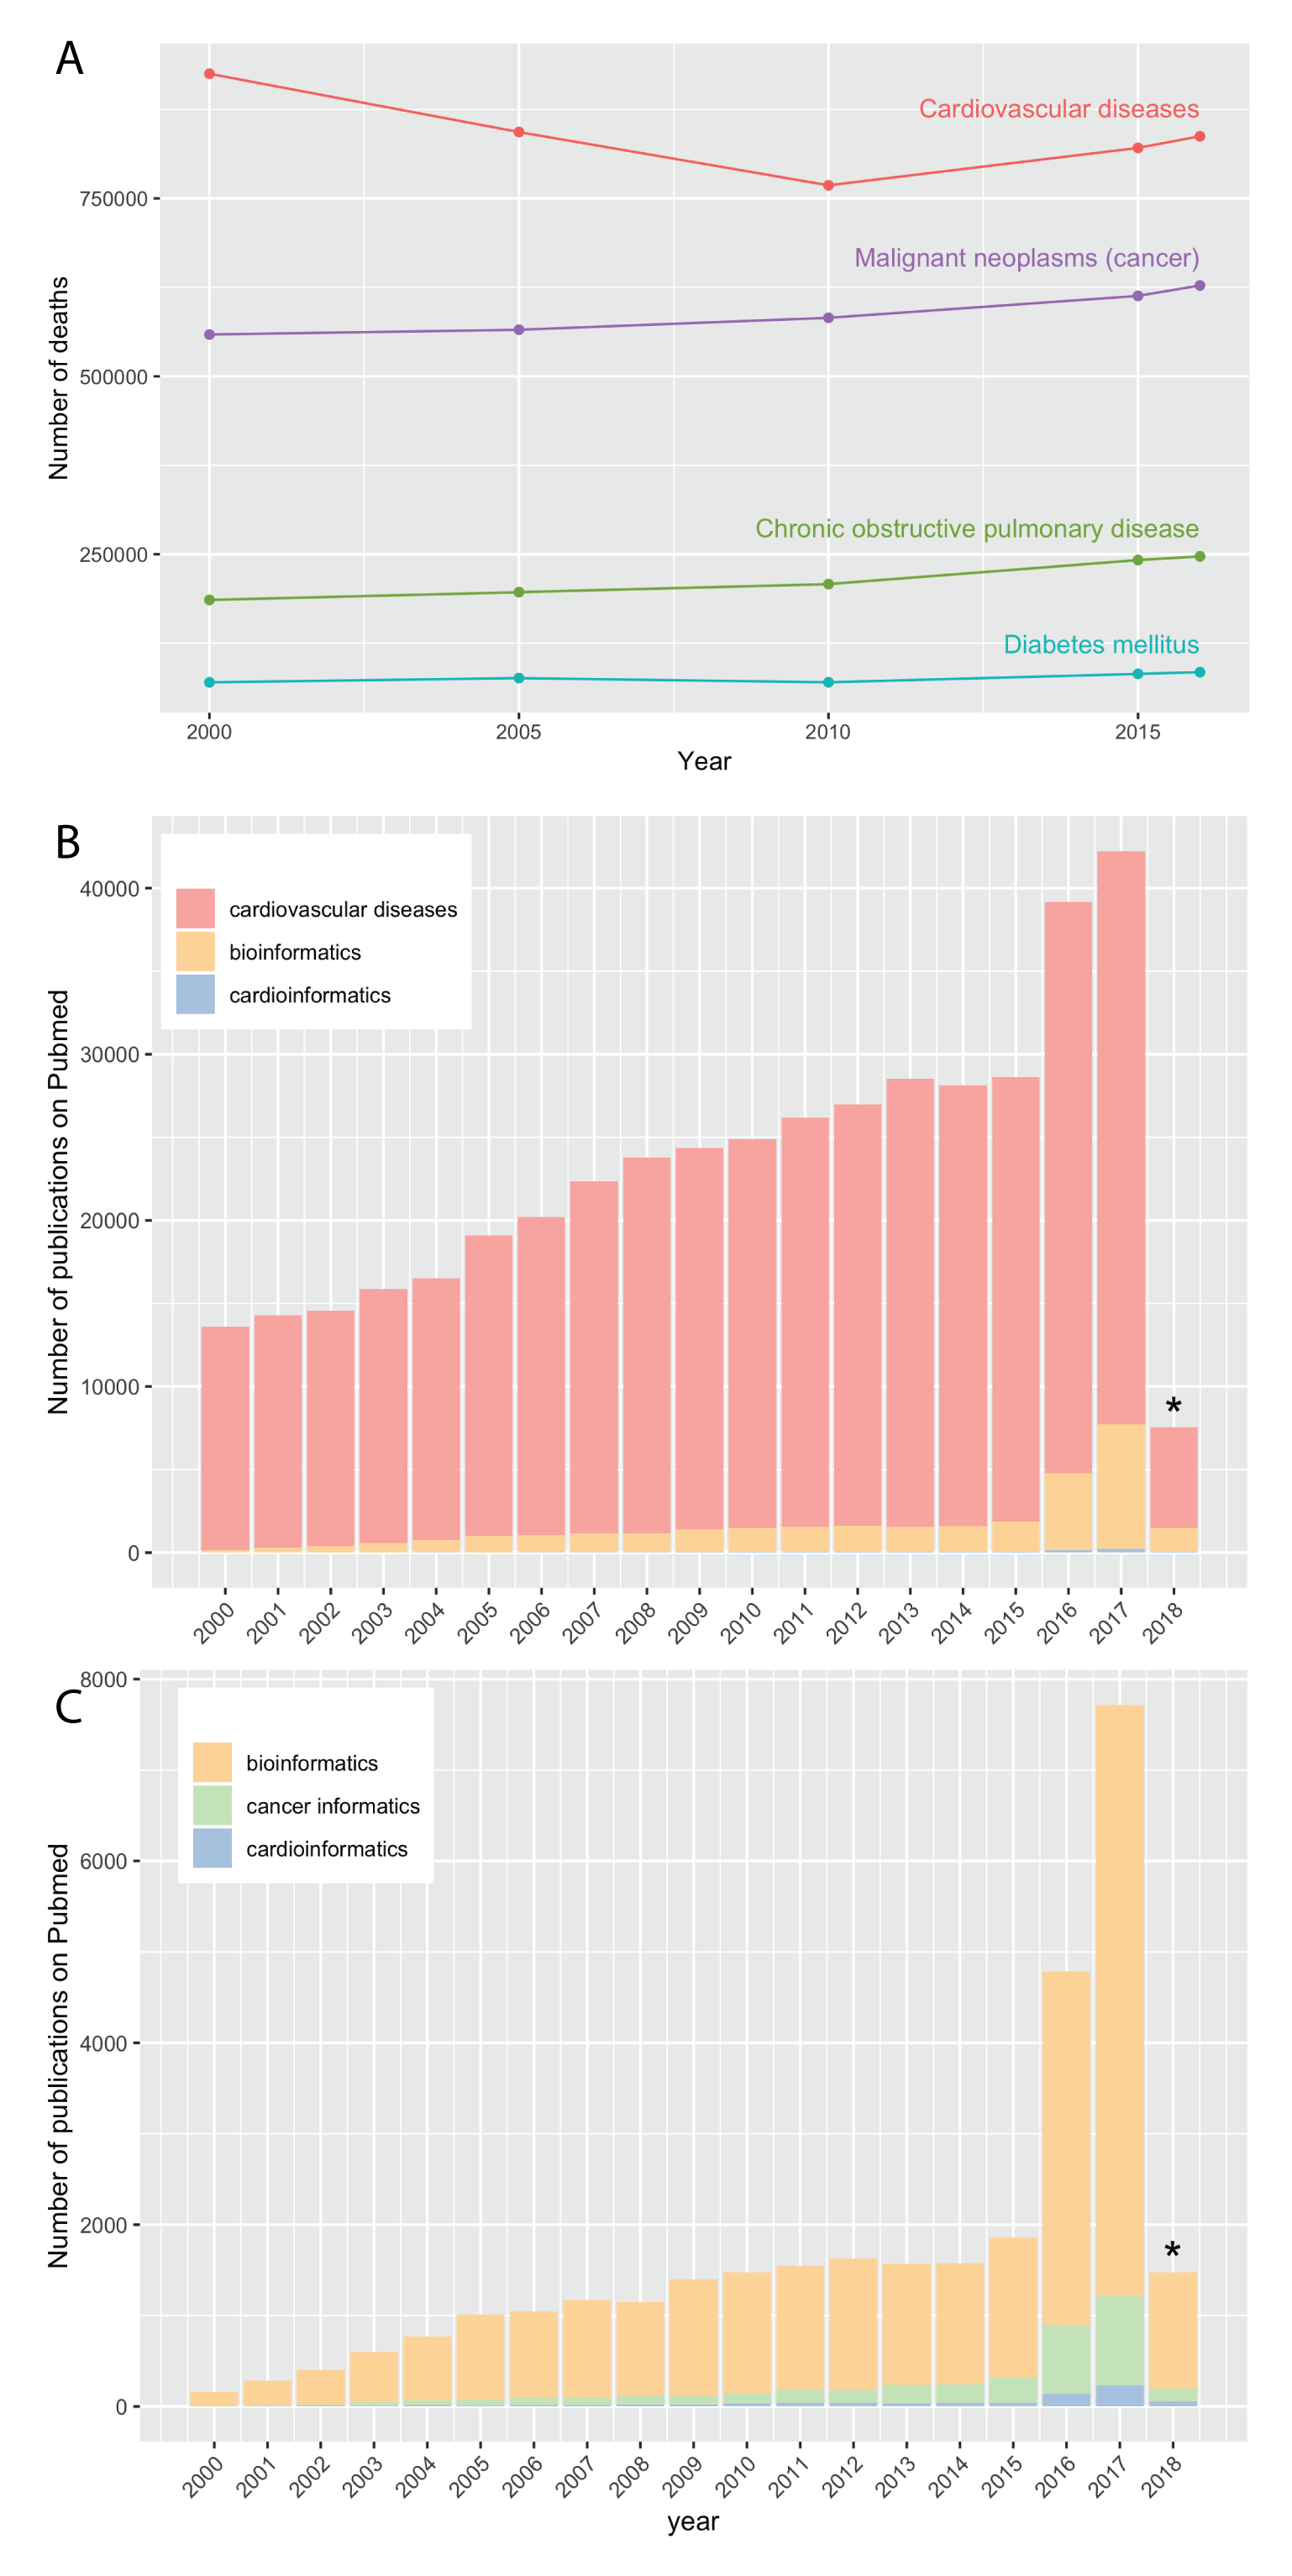
\includegraphics[width=1\linewidth]{figure1}
	\caption{\textbf{(A)} Number of deaths by Non-Communicable Diseases in the US.  Cardiovascular disease deaths have significantly surpassed cancer mortality rates since the year 2000.  \textbf{(B)} Text mining PubMed reveals that out of the total body of CVD research published in peer-reviewed journals, only a vanishingly small percentage include bioinformatics techniques or methodologies as part of the study design.  Likewise, there are far more CVD papers released annually than bioinformatics papers (in any domain area, not just CVD), highlighting the tremendous momentum and volume of new research results published in the CVD field.  Nevertheless, only a small percentage of that total CVD literature includes bioinformatics techniques.  \textbf{(C) Relative to the total pool of bioinformatics papers (in any field), there are far more cancer papers that utilize bioinformatics methods than CVD papers that utilize such methods.}}
	\label{fig:figure1}
\end{figure}


Among these CVD outputs, the share of bioinformatics research has remained modest -- at least relative to comparable work done in cancer biology (Figure \ref{fig:figure1}C). While bioinformatics is at the center of precision medicine \citep{Gomez-Lopez:2017:Precision} and cardiovascular research is at the forefront of existing precision medicine initiatives, including recent Chan Zuckerberg Biohub funding for CVD projects such as ``Multi-scale deep learning and single-cell models of cardiovascular health", the field of cardioinformatics is still in its early days with ample opportunities to benefit from cutting-edge data science techniques and machine learning (ML) methodologies, as has been the case in oncology.  Even now, the application of ML is recognized as indispensable in many aspects of cardiology \citep{Shameer:2017:Translational,Shameer:2018:Machine} and, therefore, given the availability of high-peformance ML implementations, cardioinformatics is better positioned to tackle domain-specific questions and develop clinical applications to enhance medical imaging, CVD risk prediction models, among other active research areas. Likewise, natural language processing (NLP) is a branch of artificial intelligence that can help improve large-scale CVD data collection and its organization relevant to different types of CVD information found in both literature and dataset repositories, including consortium efforts.  Recently, the American Heart Association (AHA) Institute for Precision Cardiovascular Medicine partnered with Amazon Web Services to provide a variety of grant funding opportunities for testing and refining artificial intelligence and machine learning algorithms using healthcare system data and multiple longitudinal data sources to fund research that improves our understanding of all CVD data related to precision medicine.  Therefore, we expect that grant funding initiatives such as these will gradually begin narrowing the gap between cardioinformatics and cancer research in terms of the availability of improved computational tools, infrastructure, and analysis resources.  Some recent trends in this direction include large-scale infrastructure and knowledge portal development \citep{Kass-Hout:2018:American, Khomtchouk:2018:HeartBioPortal, Broad:NA:Cardiovascular, Broad:NA:Cerebrovascular} for working with CVD data, as well as population-wide multi-omics initiatives such as the NHLBI Trans-Omics for Precision Medicine (TOPMed) Consortium \citep{NHLBI:2014:TransOmics} for integrating whole-genome sequencing (WGS) and other -omics data (e.g., metabolic profiles, protein and RNA expression patterns) with molecular, behavioral, imaging, environmental, and clinical data.  In this review, we highlight these contemporary opportunities and perspectives for CVD genomic and precision medicine research, introduce the bountiful resources available and propose ways to advance this field further by promoting a culture steeped in computation vis-\`{a}-vis modern bioinformatics methodologies.


\section*{The democratization of data and the rise of knowledge bases}

The last few years have seen a meteoric rise in the availability of computational resources and infrastructure that provide access to aggregate genetic data and genomic summary results to facilitate rapid and open sharing of individual level data and summary statistics pertinent to various biological diseases and data types.  One of the early pioneers of web-based knowledge portals has been a Memorial Sloan Kettering Cancer Center resource called cBioPortal \citep{Cerami:2012:cBio,Gao:2013:Integrative}, which provides intuitive visualization and analysis of large-scale cancer genomics datasets from large consortium efforts such as TCGA \citep{TheCancerGenomeAtlasResearchNetwork:2013:Cancer} and TARGET \citep{Koscielny:2017:Open} as well as publications from individual labs.  Other major players in the cancer knowledge base arena include the National Cancer Institute's Genomic Data Commons (GDC) Portal \citep{Grossman:2016:Shared,Jensen:2017:NCI}, which provides full-download and access to all raw data (e.g., mRNA expression files, full segmented copy number variant files, etc.) generated by TCGA and TARGET.  In addition, resources such as the Broad Institute's Single Cell Portal \citep{Broad:NA:Single} provide an unprecedented view into the biology of cancers like glioblastoma at a single-cell sequencing level.    
	
More recently, the Knowledge Portal Network Group at the Broad Institute has begun implementing a wide variety of complex disease knowledge bases focused on type II diabetes, sleep disorders, cardiovascular and cerebrovascular diseases.  The purpose of these resources is to aggregate and store statistical data for billions of genetic variants and organize them to be rapidly queried and visualized by biologists, statistical geneticists, pharmaceutical researchers, and clinicians to find genetic associations, treatment targets, etc.  Other such knowledge bases focused on exploring large-scale genetic association data in the context of, for instance, drug/treatment targets include the OpenTargets initiative \citep{Koscielny:2017:Open}, which is a public-private venture that generates evidence on the validity of therapeutic targets based on genome-scale experiments and analysis.  Similarly, the Accelerating Medicines Partnership-Alzheimer's Disease (AMP-AD) Target Discovery and Preclinical Validation Project has developed an AMP-AD Knowledge Portal to help researchers identify potential drug targets to accelerate pre-competitive Alzheimer's disease treatment and prevention \citep{NIA:2015:AMP}.  
	
	In addition to these various genetic association efforts, CVD knowledge bases such as HeartBioPortal \citep{Khomtchouk:2018:HeartBioPortal} have begun integrating gene expression information with genetic association information, motivated by the stimulus that transcriptomic data provide powerful insights into the effects of genetic variation on gene expression and alternative splicing in both health and disease.  Such large-scale integrative multi-omics efforts now also extend beyond academia into biotech startup companies such as Quiltomics, Omicsoft, Omics Data Automation, Occamzrazor, NextBio, BenevolentAI, Insitro, Researchably, etc. -- many of which have successfully been acquired by larger biotech companies such as Illumina, Qiagen, etc.  Therefore, the biological data science world has started moving progressively closer towards large-scale integration of knowledge bases, rather than just individual studies or datasets.    


		\begin{figure*}[!tpb]
		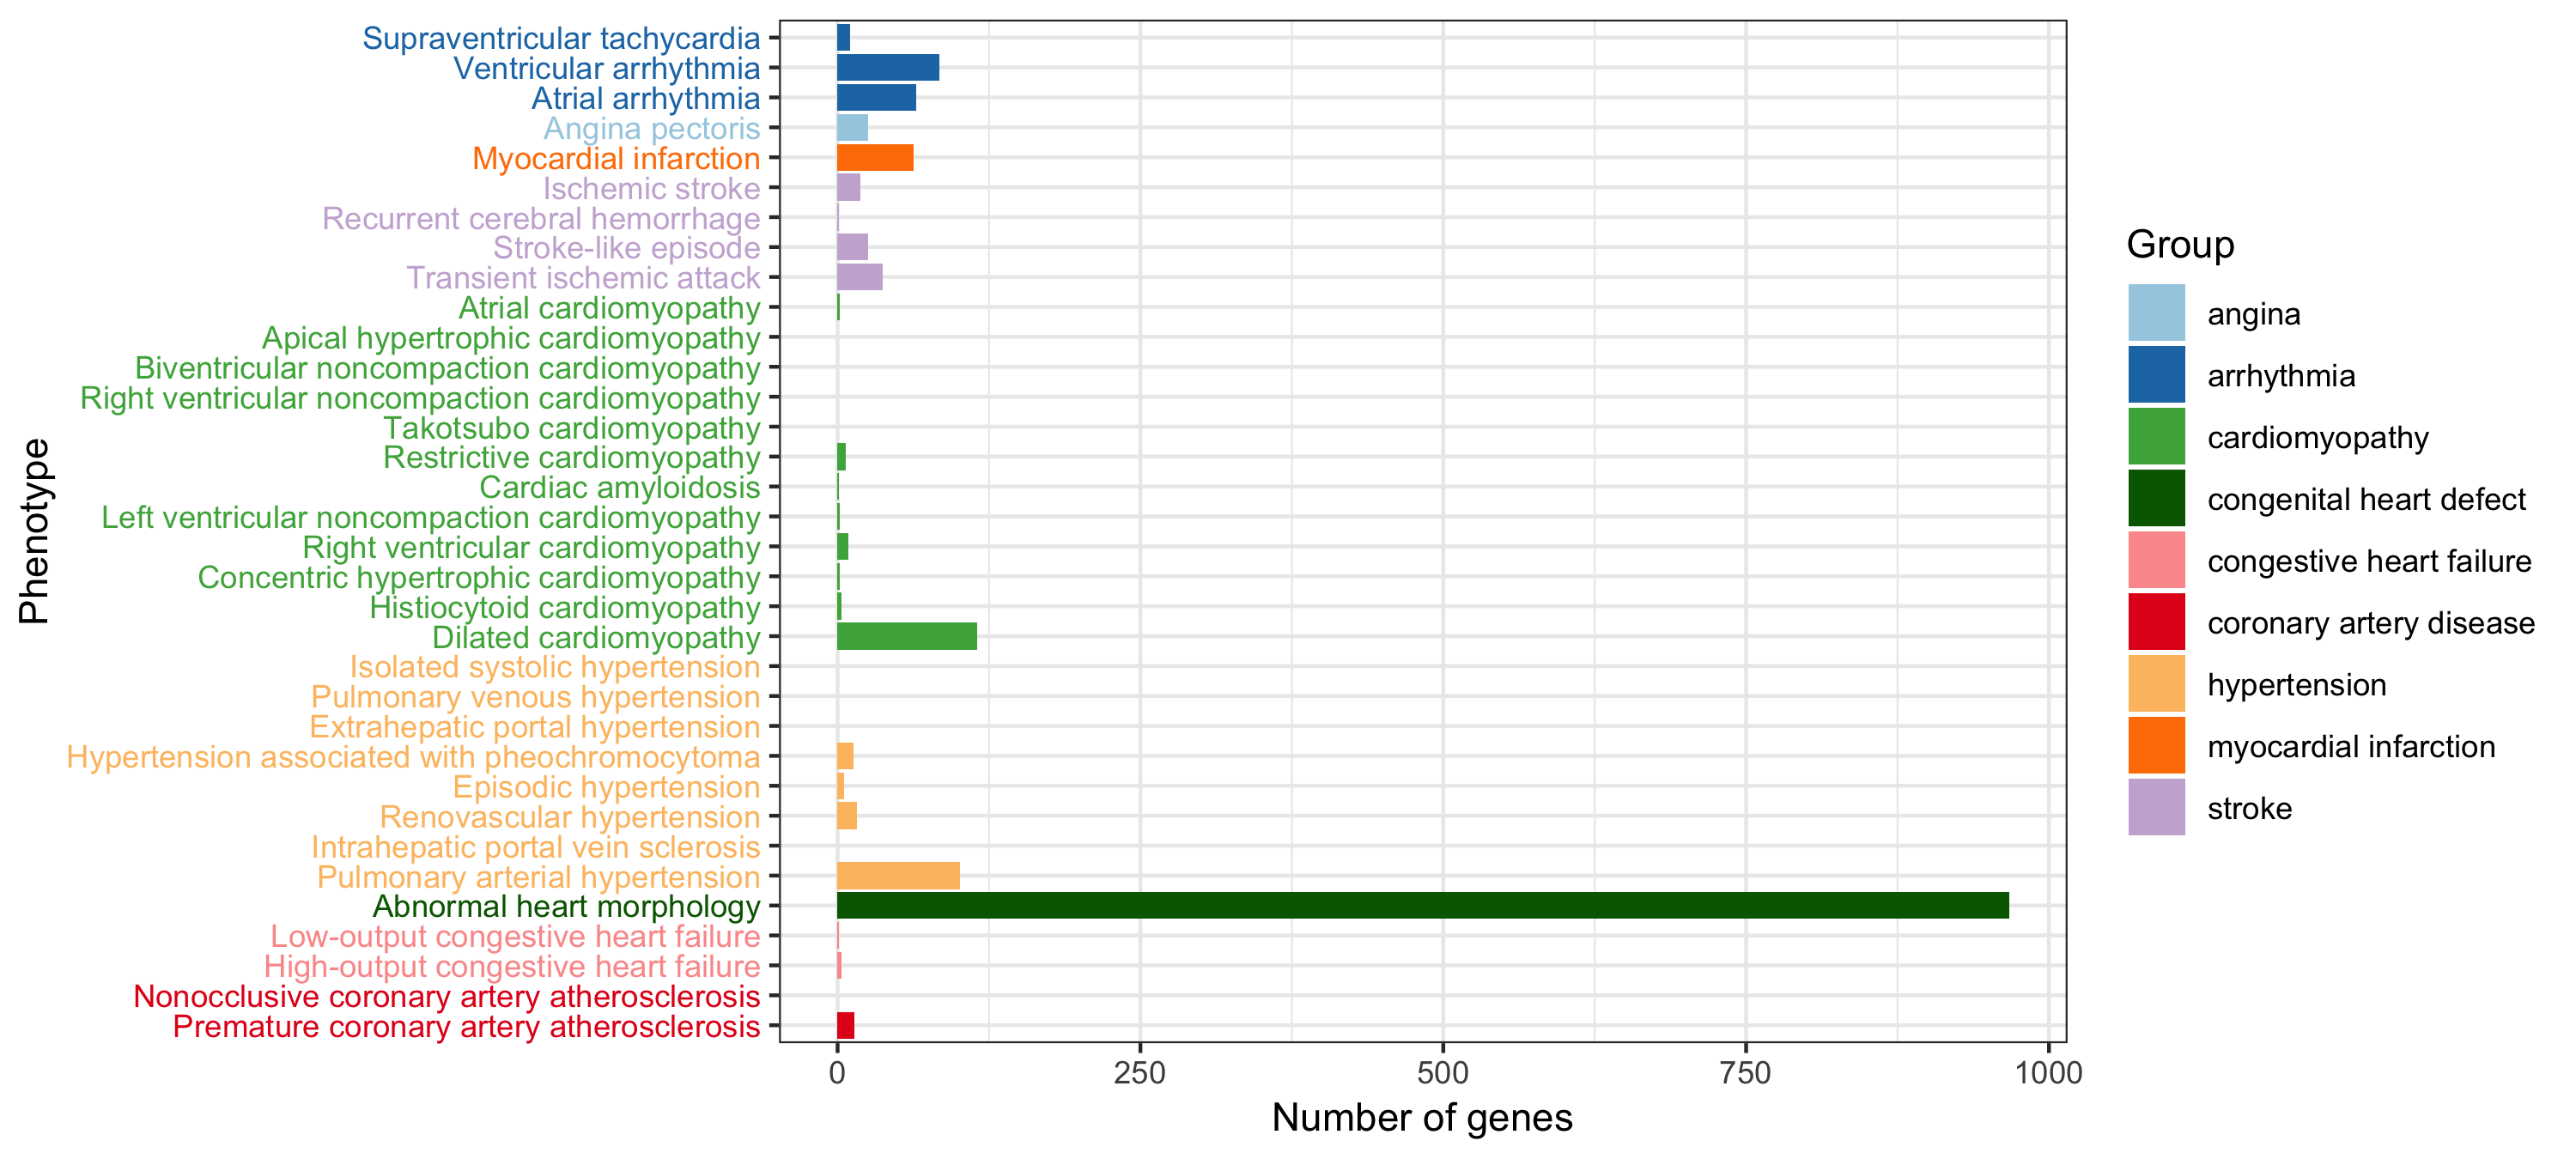
\includegraphics[width=1.\linewidth]{hpo-gene-count}
		\caption{The number of genes associated with \emph{``Abnormality of the cardiovascular system"} (HP:0001626) as reported in the Human Phenotype Ontology \citep{Kohler:2014:Human},
			 with phenotype annotations pooled from OMIM \citep{McKusick:2018:OMIM} , Orphanet \citep{INSERM:1997:Orphanet}  and DECIPHER \citep{Firth:2009:DECIPHER}.}
		\label{fig:hpo_gene_count}	
	\end{figure*}
	
	
	
	
	\section*{Complexity of CVDs}  % the problems
	\subsection*{The number of actors}
	
	% large number --> small effects
	% large number --> more interactions, intra and inter-pathways
	% 
There is a certain genetic component in all major categories of heart disease (Figure \ref{fig:hpo_gene_count}).  As more studies are published, the number of genes found associated with a disease has also increased and, in most cases, gone beyond a few genes that could be described in a single-page table or diagram.  Dilated cardiomyopathy (DCM), the most common cause of heart transplantation, is a vivid example of how causal variants and their corresponding genes were discovered over the years.  In a recent review \citep{Burke:2016:Clinical}, 16 disease-causing genes were compiled, along with an additional 41 putative genes.  Meanwhile, the NHGRI-EBI GWAS Catalog \citep{MacArthur:2017:new} and annotations on Human Phenotype Ontology \citep{Kohler:2017:Human} suggested a much larger number of genes associated with this condition, 69 genes and 115 genes, respectively.  Clinical application has been keeping up, with a typical commercial gene panel for DCM genetic testing covering 50 genes on average, and 111 in total \citep{McNally:2017:Dilated}.  These numbers suggest the need for more bioinformatics analyses to gain insights into this condition and other CVD conditions that are equivalently complex.  Since it is reasonably expected that when more genes are involved in a disease, the individual effect exerted by each gene gets smaller, these constantly expanding gene panels suggest that the risks conferred by mutations in a single gene are less likely to be indicative of the disease risk.  For example, one recent study asserted the negative correlation between minor allele frequency and the effect size across all tissues (liver, skeletal muscle, adipose tissue, atherosclerotic aortic root, artery and blood) in the Stockholm-Tartu Atherosclerosis Reverse Networks Engineering Task study (STARNET) \citep{Franzen:2016:Cardiometabolic}.  From a research perspective, these findings imply that the quest of pinpointing causal variants is getting more challenging, because testing the variant-phenotype association on small-effect variations requires a much larger number of samples for sufficient power, or critically different methods of statistical testing and inference. \hl{(Tim, would you like to include a word or two on Mendelian randomization and instrumental variable analysis here?)}
	
	
Besides the increasing difficulty of discovering these genes, modeling their effects poses its own unique set of challenges. With a potential interaction between every pair of genomic features, be they genes or regulatory sequences, the number of such interactions increase quadratically with the number of actors, leading to the combinatorial explosion of states that a biological system can assume.  Ethnicity and ancestry-specific differences add a further layer of complexity. \hl{(Tim, would you care to elaborate more here?)}
	
The number of genes or regulatory elements contributing to CVD risks will likely inflate beyond those directly associated with diseased traits, due to the highly interconnected wiring of biological pathways.  For instance, independent research in aging has unraveled the intertwined relationship between heart disease and longevity pathways \citep{North:2012:Intersection}.  With age being the most important factor in constituting cardiovascular disease risk \citep{Steenman:2017:Cardiac}, it is unavoidable that these longevity genes will be involved in future analyses of CVD genetics. The genetic scope of these diseases may be enlarged even further to include most of the genome, under the recently proposed omnigenic model for complex traits, in which most heritability is explained by peripheral genes outside of the core pathways \citep{Boyle:2017:Expanded}. Such expansion calls for a paradigm shift from additive effects of multiple genes to the interactions between them, from the physical genes to the "eigen-genes" that represent biologically functional modules \citep{Weiss:2012:Good}.
% From a historical perspective, when thousands of loci were found to be involved in a single disease, the paradigm shifted from additive effects of multiple-genes to the interactions between them, turning the focus from physical genes to the "eigengenes" that represent biologically functional modules \citep{Weiss:2012:Good}. The ability to view and compute on biological systems as a whole allows one to focus on the effects of a drug without the mechanistic knowledge of individual actors and their interactions. From a research perspective, such approaches are also helpful for understanding a system by ways of its response to external stimuli. 
	
As with other complex diseases, missing heritability has been a long-standing puzzle in cardiovascular disease \citep{Manolio:2009:Finding}. Despite the early successes in pinpointing the causes of several monogenic diseases, the large body of genome-wide association studies have defied many widely-held beliefs about genetic variants in humans, hinting at various directions to search for the missing heritability.  The most trivial situation where inherited risk is not fully accounted for is when the variants are simply too rare to be detected with sufficient power. One addresses this issue by collecting more samples or improving statistical tests.  This reason has driven a lot of efforts to enlarge and diversify the study population, where the availability of a large number of genomes and exomes are currently enabling the search for rare variants, as embodied by ongoing large-scale consortium efforts such as the Million Veterans Project \citep{Gaziano:2016:Million}, ExAC then gnomAD \citep{Lek:2016:Analysis}, and TOPMed \citep{NHLBI:2014:TransOmics}. The other directions to search for missing heritability require one to move beyond the exome and genome, as discussed in the next section.
	
	
	%does it help to have too many variants in a genetic risk score?
	
	
\subsection*{The diversity of actors in an era of trans-omics}

\subsubsection*{From single-nucleotide to structural variations}
	
	%\begin{figure*}[!tpb]
		%	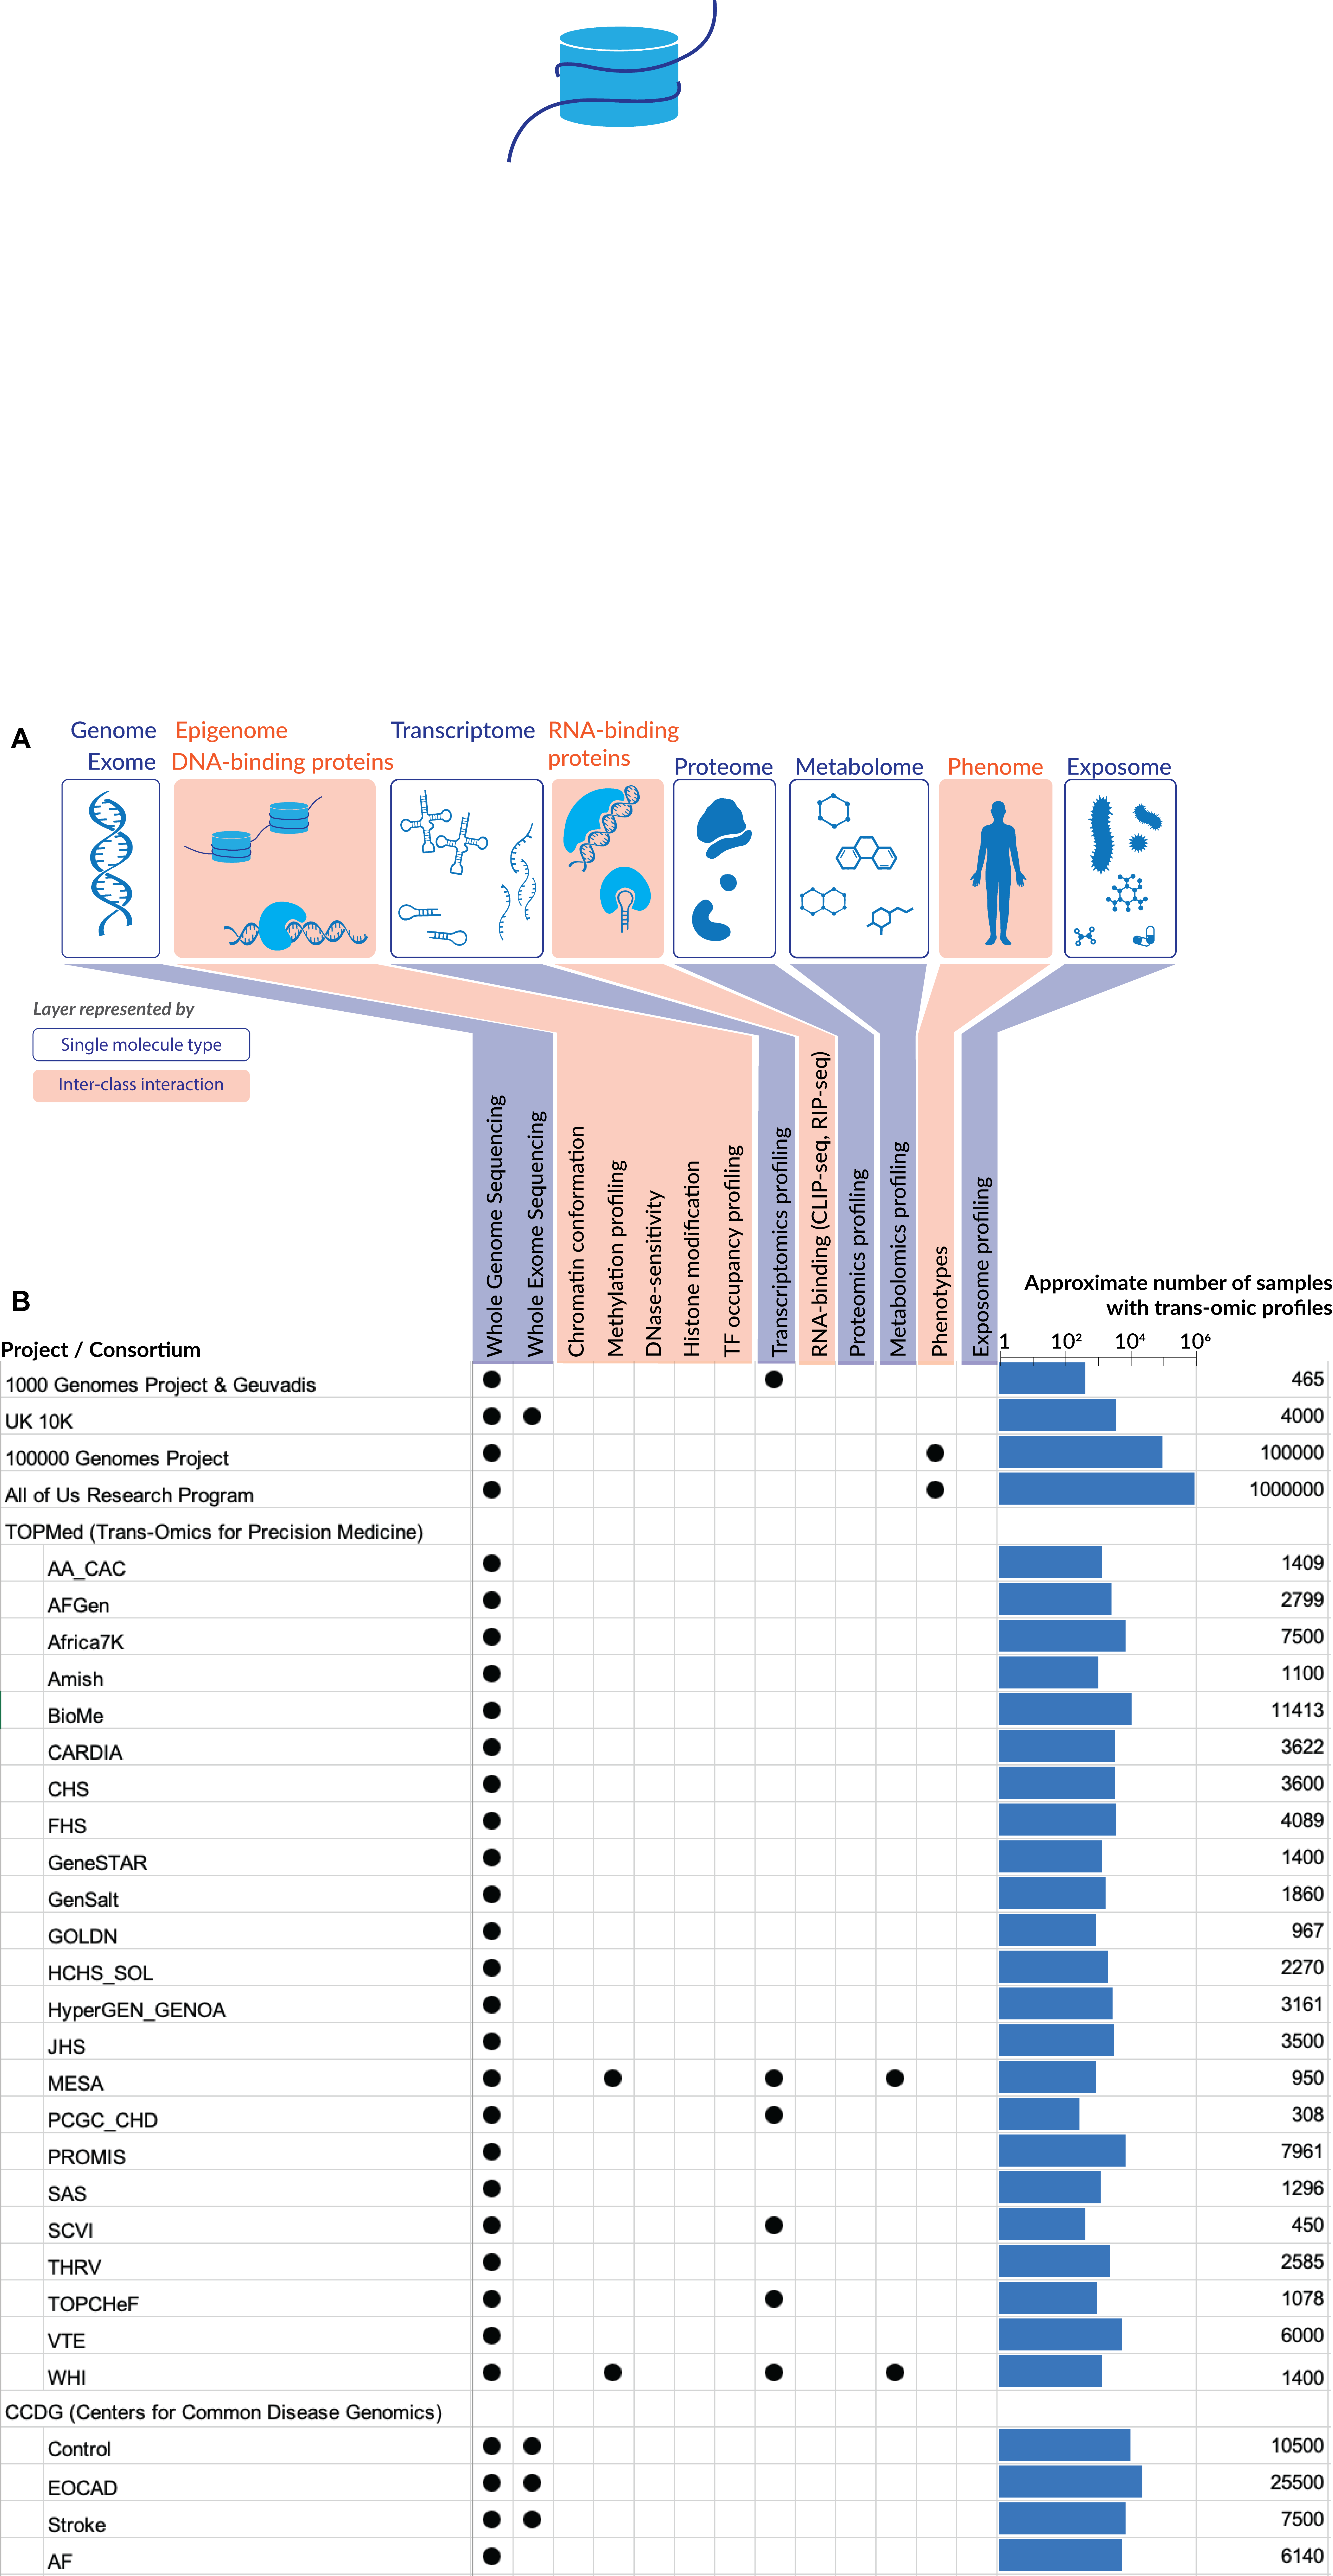
\includegraphics[width=1\linewidth]{multiomics}
		%\rule{2cm}{2cm}
		%\caption{PLACE HOLDER - layers of omics data and the corresponding molecular assays. \comment{Genome, epigenome, transcriptome, proteome, metabolome, microbiome, exposome}}
		%\label{fig:multiomics}
	%\end{figure*} 
	
	% Our understanding of CVD has been critically limited by the technical capability in characterizing various molecular fractions of a cell \hl{(this sounds like the perfect moment to discuss the impact that single-cell sequencing has had in CVD)}.
	Historically, genome-wide association studies were predominantly conducted on single-nucleotide polymorphisms (SNPs) thanks to the availability of easy-to-produce SNP microarrays. Such technologies have clearly enriched our knowledge base of single nucleotide variants, while leaving structural variations poorly understood. There are now 660 million SNPs documented in the dbSNP database \citep{NCBI:2018:dbSNP}, compared to 4.6 million structural variations in the DGVa (Database of Genomic Variants archive \citep{EMBL-EBI:2018:Database}, which also includes studies annotated by the NCBI-hosted database of structural variants, dbVar \citep{NCBI:2018:dbVar}).  Structural variation (SV) databases such as dbVar and DGVa are in fact storing each study-publication individually instead of cataloging structural variations into data entries. Although the current knowledge base of structural variations is not sufficient to create reference entries of SV, the map of SV from 1000 Genomes Project \citep{Sudmant:2015:integrated} has enabled further studies of the role of SV in cardiac diseases, suggesting the potential impact of SV on the transcriptional regulation of cardiac genes expressed in the heart \citep{Haas:2018:Genomic}. As envisioned, structural variations might be one of the promising lands to look for the missing heritability in CVD \citep{Eichler:2010:Missing}.  To this end, projects like TOPMed contain a Structural Variant Working Group to call copy-number variants (CNVs) within TOPMed, and they have begun incorporating large-scale multi-ancestry studies spanning diverse types of sequencing data from both European and non-European race/ethnic groups.  For instance, the Women's Health Intiative (WHI) study \citep{NHLBI:1991:Women} within TOPMed currently includes WGS, RNA-seq, metabolomics, and methylomics data.  Likewise, the Multi-Ethnic Study of Atherosclerosis (MESA) study \citep{Bild:2002:MultiEthnic} within TOPMed includes WGS, RNA-seq, metabolomics, proteomics, and methylomics data across a variety of multi-ethnic communities (white, Hispanic, African-American, and Asian).  Specifically, MESA investigates the characteristics of subclinical cardiovascular disease (disease detected non-invasively before it has produced clinical signs and symptoms) and the risk factors that predict progression to clinically overt cardiovascular disease or progression of the subclinical disease.  In general, improved risk prediction methods such as polygenic risk scores are being used to improve our ability to predict future CVD events \citep{Goldstein:2014:Simple}, and have demonstrated the ability to serve as a biomarker that is predictive of clinical outcomes to the same degree as some traditional cardiovascular risk factors (e.g., cholesterol, smoking, obesity, etc.) \citep{deVries:2015:Incremental}. 
	
	\begin{figure}[!tpb]
		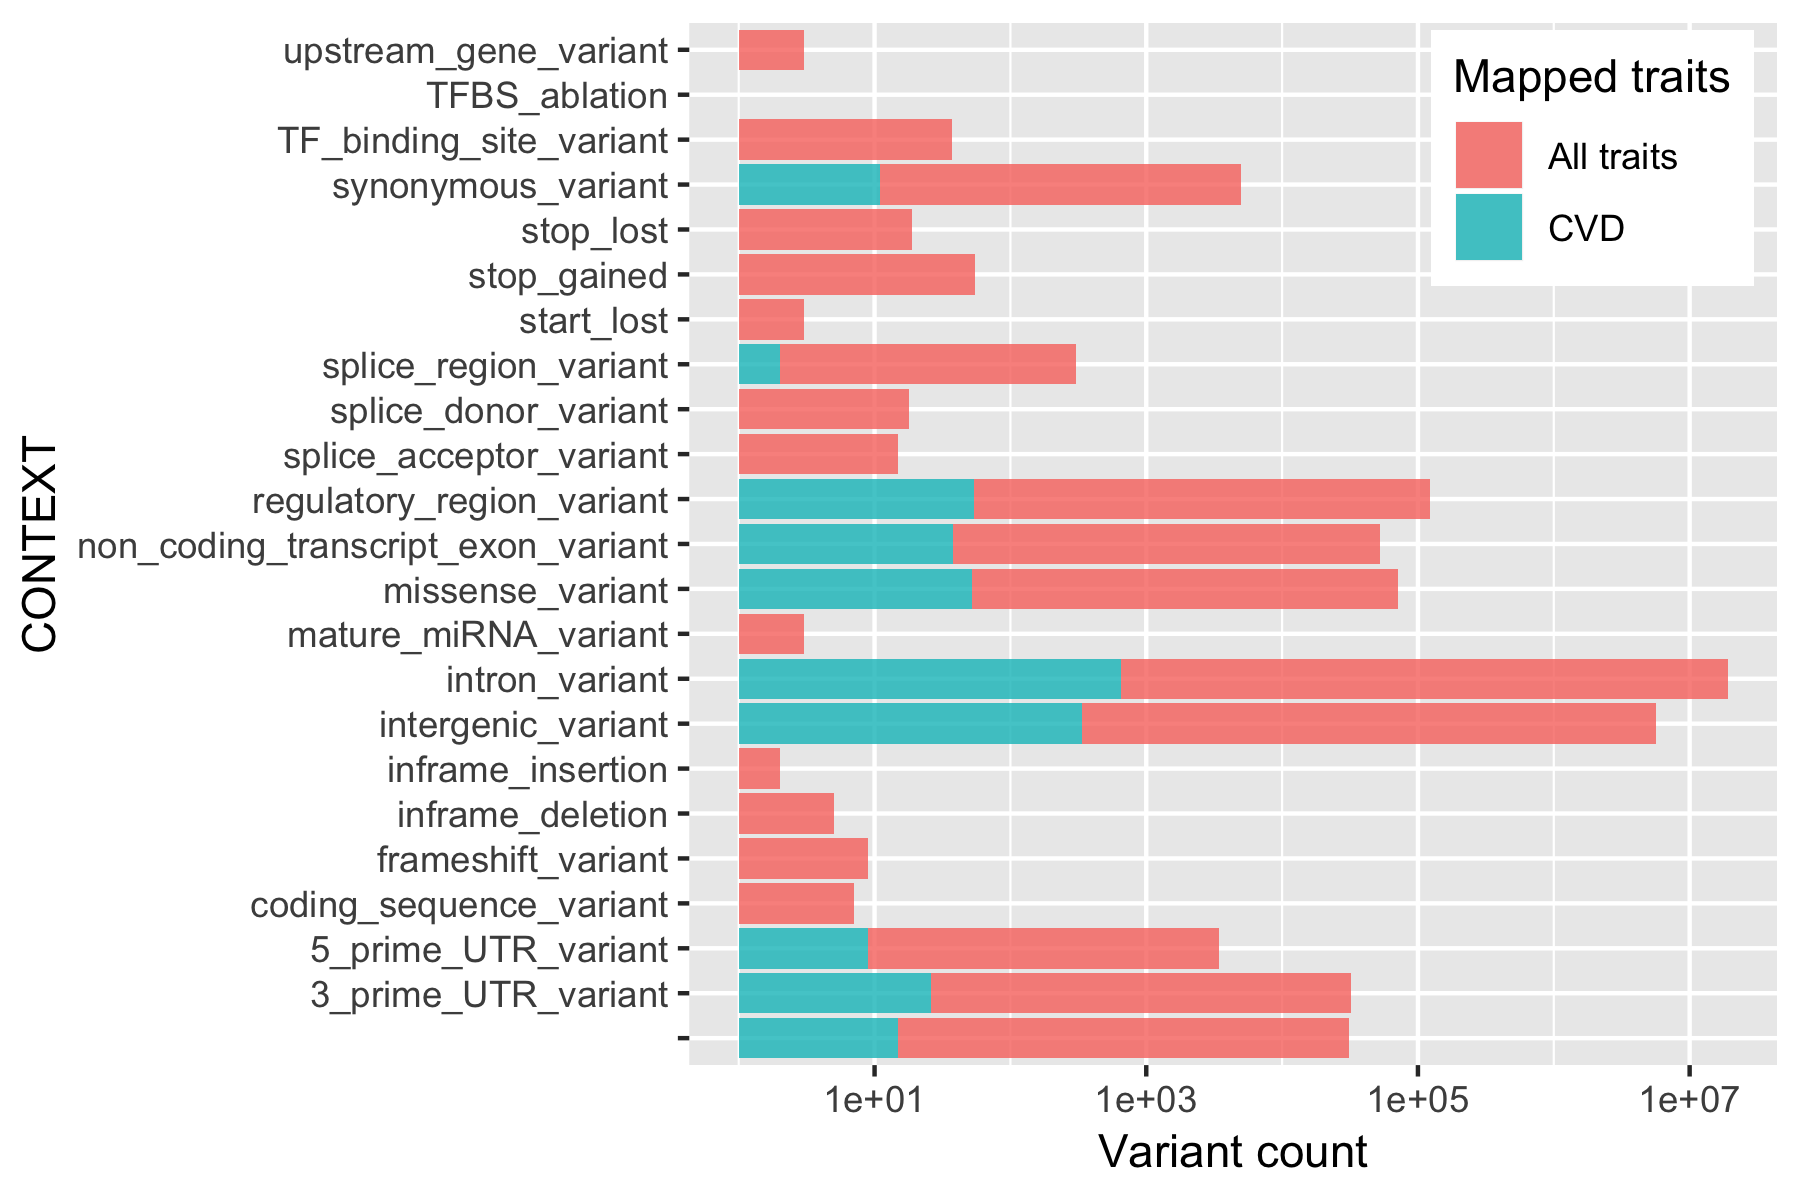
\includegraphics[width=1\linewidth]{variant_contexts}
		\caption{Distribution of SNPs that have been associated with a phenotypic trait in the human genome. The associations are downloaded from NHGRI-EBI GWAS Catalog in which only those with p-value less than $10^{-5}$ were retained.}
		\label{fig:variant_context}
	\end{figure}
	

\subsubsection*{From coding to non-coding regions}	
	% non-coding
	When array-based genotyping was gradually replaced by next-generation sequencing, the cost of sequencing an \textit{exome}, the protein-coding part of a genome, became much more affordable and enabled the collection of more than 60000 exomes \citep{Lek:2016:Analysis}. Using this dataset, \cite{Walsh:2017:Reassessment} found that many genetic variants associated with various cardiomyopathies turned out to be equally common in clinical cases as in the control population. Genes that were consistently included on genetic testing panels for DCM such as MYBPC3, MYH6, SCN5A, etc. turned out to contribute much less etiology than previously thought, in consideration of their frequency in the control population.  In fact, the rationale for prioritizing the sequencing of exome over that of the entire genome was originally based on a regularly cited statement that the exome harbors 85\% of disease-causing variants \citep{Antonarakis:2001:nature}.  However, this number is an outdated estimate from 1995.  Specifically, it is found that among the variation-phenotype associations curated in the NHGRI-EBI GWAS Catalog \citep{MacArthur:2017:new}, a large fraction of variants tend to occur in non-protein coding regions such as intronic, intergenic, and splice junctions (Figure \ref{fig:variant_context}). The distribution of CVD-associated variants are in fact highly similar to that of all variants across the human genome. Previous studies also asserted the prevalence of regulatory regions among variants associated with cardiometabolic risk \citep{Franzen:2016:Cardiometabolic}, as well as many other complex traits \citep{Pickrell:2014:Joint}. As an unprecedented amount of whole-genome sequencing data become available from large-scale genomic projects such as 1000G  \citep{1000G:2015:global}, TOPMed \citep{NHLBI:2014:TransOmics}, and CCDG \citep{NHGRI:2016:CCDG}, we are poised to learn more about this dark matter in the human genome and how it works in complex diseases.

\subsubsection*{Beyond genetics: epigenetics and gene-environment interplay}	
	%epigenetics
	Cardiovascular risks can be conferred with heritable changes in gene expression that occur without underlying alterations in the DNA sequence, collectively studied as epigenetics. Epigenetic processes traditionally involve chromatin remodeling, DNA methylation, a wide range of histone modifications including acetylation, methylation, phosphorylation, ubiquitylation, sumoylation and biotinylation, and are now encompassing a loosely-defined group of processes mediated by the class of long noncoding RNAs (lncRNA). Epigenetics plays a key role in human biology, and dysregulation in epigenetic processes is associated with the pathogenesis of cancer and many other diseases. Epigenetic mechanisms have been demonstrated to be necessary for biological programs important for a variety of cardiovascular diseases and conditions \citep{Udali:2013:Cardiovascular,AbiKhalil:2014:emerging,Muka:2016:role,Gidlof:2016:Ischemic}.
	For instance, early differential epigenomic analysis, albeit on a limited number of samples, established differentiating features in DNA methylation and histone H3 methylation between control and failing hearts \citep{Movassagh:2011:Distinct}, probing more epigenomic research in cardiovascular diseases. Following these early findings, epigenome-wide association studies are proposing a number of DNA methylation sites associated with blood lipid \citep{Irvin:2014:Epigenomewide}, body mass index \citep{Dick:2014:DNA, Wahl:2017:Epigenomewide}, heart failure \citep{Meder:2017:EpigenomeWide}, and heart attack history \citep{Rask-Andersen:2016:Epigenomewide}. It has also been found that alterations in chromatin structure could induce heart failure \citep{Rosa-Garrido:2017:HighResolution}.
	When more lncRNAs were discovered and characterized, the prevalence of these molecules in cardiovascular biology also emerged. For example, lncRNAs have been found to be implicated in coronary artery disease, myocardial infarction, cardiac hypertrophy, and other cardiovascular diseases. At least 22 lncRNAs were reportedly dysregulated in CVDs, affecting a wide range of molecular, cellular and physiological processes \citep{Das:2018:Deciphering}. With 107,039 lncRNAs detected in the human genome so far (reported by LNCipedia \citep{Volders:2018:LNCipedia}, as of November 2018), more lncRNAs are likely to be found involved in cardiovascular biology, hence promising potential therapeutic targets.
	% cardiac differentiation, histone methylation, sponge of microRNAs, apoptosis
	%angiogenesis, inflammation, macrophage activation, sarcomere development, autophagy
	Mapping the epigenome involves a highly diverse set of experimental assays. DNA methylation profiling can be done with methylation-sensitive restriction enzymes, bisulfite sequencing, or immunoprecipitation with antibodies against methylated-cytosine \citep{Bibikova:2010:Genomewide}. Histone modifications can be profiled by immunoprecipitation with antibodies specific to the modified histone of interest, essentially requiring a ChIP experiment for each of the histone modifications one wants to interrogate. Meanwhile, the noncoding RNA transcripts can be profiled with variations of RNA-seq experiments that are optimized for the target fraction of RNA. Such diversity entails significant difficulty in comprehensive profiling of the epigenome in a single experimental assay, stressing the need for re-collection and re-analysis of dispersed datasets for a more complete picture.
	
	%Epigenetic studies supplemented significant mechanistic insights to understand complex conditions  such as atherosclerosis \citep{Xu:2018:Targeting}. 
	
	%Difficulty in studying lncRNAs: low abundance level, highly tissue-specific expression. Approaches to study lncRNAs \citep{Sallam:2018:Long}
	
	%A range of functions have been reported for lncRNAs, including imprinting, scaffolding, enhancer, and molecular sponges. More research is certainly needed to obtain a complete catalog of lncRNA functions. \comment{role of non-coding RNAs and epigenetics in cardiovascular biology \citep{Sallam:2018:Long}}

	
	%environment interactions
	
	It has been known for decades that non-genetic factors play a critical role in cardiovascular health, such that a risk prediction using lifestyle variables perform much better than a gene-count score \citep{Joyner:2011:Ten}. Although such interactions are of focal interest to cardiovascular epidemiology,  the understanding of them at the molecular level has been restricted due to the difficulties in measuring the numerous agents in an exposome, i.e. all environmental exposures throughout life, including one's diet, pollutants, infections \citep{Wild:2005:Complementing}. Continual improvement of existing chemical profiling methods including mass spectronomy (MS), LC-MS, GC-MS, and their variations, has enabled the detection of hundreds of thousands of xenobiotic compounds \comment{(check for specific number on state-of-the art facility)} in human urine and blood samples \citep{Warth:2017:ExposomeScale}.
	Recent development of wearable devices can now collect real time data in a non-intrusive manner, allowing for dynamic monitoring of the exposome \citep{Jiang:2018:Dynamic}. As complex traits being heavily influenced by environmental factors, cardiovascular diseases are especially well-positioned to benefit from the advancement of exposome measurement.
	
	
    %From a molecular perspective, a phenotype can be influenced at any stage, starting from the DNA sequence, to the chromatin structures and modifications, down to RNA transcripts, proteins and metabolites \comment{Figure \ref{fig:multiomics}}. Accordingly, a gene (and its variants) may exert its effect in various modes.
	
	
	%As demonstrated earlier, the large number of studies have contributed to a larger, not necessarily more solid, body of knowledge. In the following section, we argue for the readiness and the prospect of cardioinformatics, by looking at the current infrastructure for biological data analysis and the computational methods.
	
	\section*{The extent of cardioinformatics}
	
	%\comment{This part is to introduce the achievements and on-going work in developing the infrastructure for data storage, management and sharing, thus making the case for an invest in bioinformatics analyses to capitalize on these resources.}
	
	The complexity of cardiovascular diseases calls for pushing research beyond traditional subjects and methodology of the field. CVD research is positioned to benefit from the accumulation of biological data and the active developments of infrastructure for data management and analysis.
	
	\subsection*{Accumulation of data}

	Biological data has steadily increased, in both the number of data points and the number of dimensions in each data point.
	Major classes of biological molecules including DNA, RNA and protein can now be characterized and/or quantified with high-throughput techniques. The output of these assays is essentially a giant vector on the order of $10^3$ to $10^5$ elements depending on the type of molecule and technology.
	Central repositories have been established to facilitate data sharing and re-analysis of various data types: Gene Expression Omnibus (GEO) \citep{Barrett:2013:NCBI} for gene expression data, dbGaP \citep{Tryka:2014:dbGaP} for genotypes and phenotypes, ProteomeXchange \citep{Vizcaino:2014:ProteomeXchange,Deutsch:2017:ProteomeXchange} for proteomics, MetabolomeXchange for metabolomics .
	GEO has accumulated an immense number of assays, effectively increasing the number of data points available for future studies.
	In GEO, CVD publications alone have contributed more than 2000 microarray datasets for expression profiling, and about 900 high-throughput sequencing datasets for various purposes (Figure \ref{fig:geo-assay}). Expression profiling by high-throughput sequencing, i.e. mRNA-seq assays, are often coupled with another profiling technique, for example, to provide functional read-out of transcription factor binding profiled by ChIP-seq.
	In dbGaP, where human genotype-phenotype data are deposited, CVD research has collected data on 658,305 subjects, 16,786 (2.5\%) of whom had consented for the data to be employed for general research (Table \ref{tab:dbgapSubject}) (See Supplementary information for a comprehensive list of CVD studies deposited on dbGaP.) Similarly, ProteomeXchange and 
	ProteomeXchange
	
	In addition to the above central repositories for established and popular experimental methods, smaller databases with narrower focus are budding. For instance, chromatin structure data from 3C, 4C, 5C and Hi-C experiments have been collected in dedicated databases such as 3CDB \citep{Yun:2016:3CDB} and 4DGenome \citep{Teng:2015:4DGenome}. Non-coding RNAs are being added into databases such as lncRNAdb \citep{Quek:2015:lncRNAdb}, NONCODE \citep{Fang:2018:NONCODEV5}, and LNCipedia \citep{Volders:2018:LNCipedia}.  Similar to structural variations, data in these under-explored areas are actively annotated to enable building reference sets and promise to make the picture of CVD as a spectrum of complex diseases more complete.

	%\begin{table}[!t]
	%	\processtable{Number of samples available on GEO that are of potential use of cardioinformatics research, including those deposited by CVD studies and non-CVD studies.\label{tab:geoSamples}} {\begin{tabular}{@{}llll@{}}\toprule 
	%			molecule &non-CVD studies & CVD studies \\ \midrule
	%			genomic DNA &            440 &        8525  \\
	%			polyA RNA &             89 &         392  \\
	%			total RNA &           2974 &       39540  \\
	%			other &             NA &           5  \\
	%			protein &             NA &           3  \\ \botrule
	%	\end{tabular}}{This is a footnote}
	%\end{table}
		
	\begin{figure*}[!tpb]
		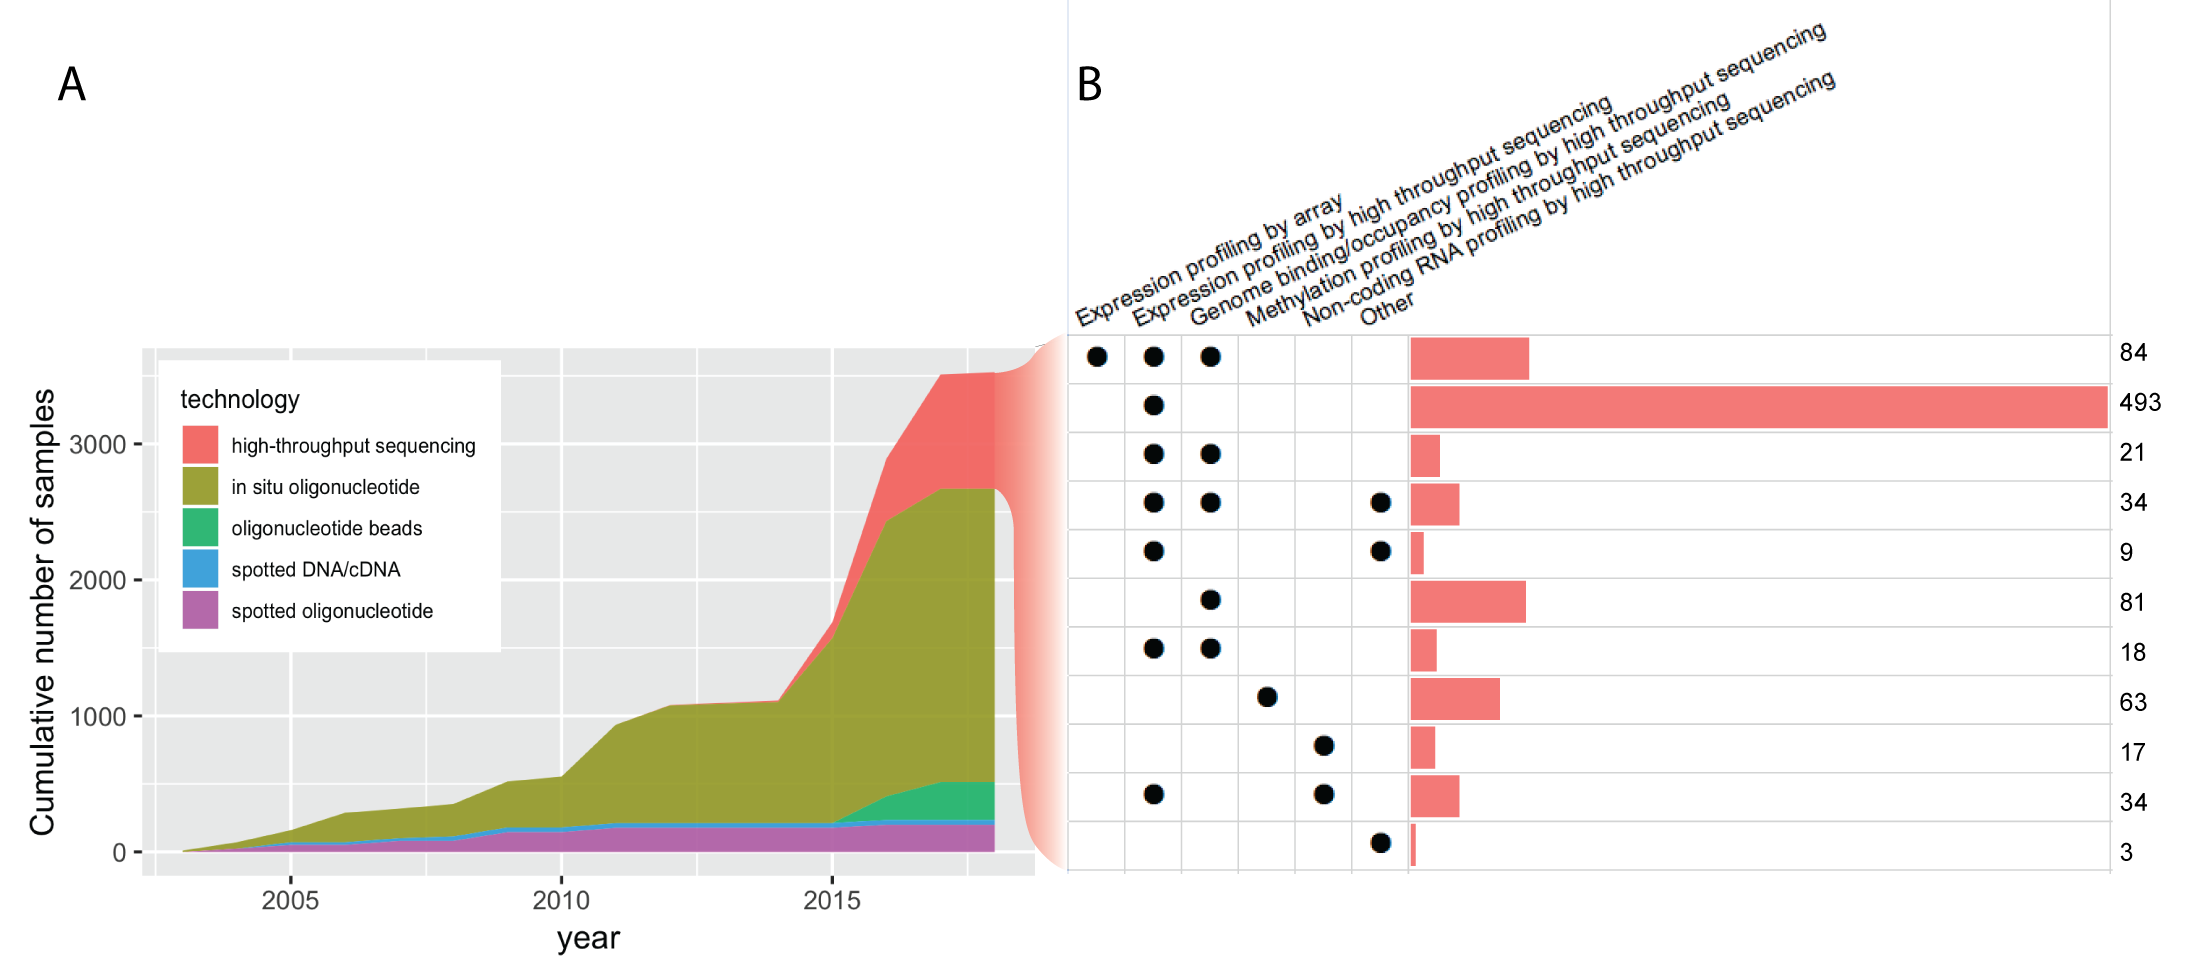
\includegraphics[width=1\linewidth]{assay-count-cardio}
		\caption{(\textbf{A}) The cumulative number of molecular assays (i.e. unique combinations of biosample, study and platform) deposited on GEO by cardiovascular research. (\textbf{B}) Breakdown of high-throughput sequencing assays by the type of study.  \label{fig:geo-assay} Note that to avoid excessive over-counting of irrelevant samples such as those from plants or unrelated model organisms, we only counted samples deposited with a Pubmed ID pointing to a cardiovascular study. Surveys were done on the GEOmetadb database \citep{Zhu:2008:GEOmetadb} updated on 2018/11/17.}
	\end{figure*} 
		    
	Being dominant in biomedical research are genotype-phenotype data in which variations are assayed on pre-defined array of SNPs while phenotype is usually recorded as a binary trait, i.e. control vs disease state. This type of data has enabled the discovery of more than 80000 variation-phenotype associations by means of genome-wide association studies (GWAS).
	When deeper phenotype data, such as blood lipid tests, diagnosis (ICD) codes, etc., is available, phenome-wide association studies (PheWAS) can be done. This phenotype data is especially rich in electrical health records (EHRs) which are abundant from clinical care institutions, enabling powerful analyses when coupled with omics data, as discussed by \cite{Denaxas:2015:Big, Wu:2017:Omic} and exemplified by  \cite{Dewey:2016:Distribution,Li:2018:Decoding}.
	EHR data, while abundant, is unstructured and requires significant processing to become useful for research. Other equally  extensive but more structured sources of phenotype data are available from pre-meditated data collection programs such as the Million Veteran Program (MVP) \citep{Gaziano:2016:Million}, the UK Biobank \citep{Collins:2012:Biobank} and many other national biobanks. (For a comprehensive list of human genotype-phenotype data, please see the review by \cite{Brookes:2015:Human}.)
	Recent research programs have started to put more focus on high-throughput assays that result in a comprehensive cross-section of biological molecules (DNA, RNA and protein) and their interactions.  Figure \ref{fig:trans-omics} highlights the large data sets that are or will be available for cardiovascular research. It is clear that assays for DNA sequence, including whole-genome sequencing and whole-exome sequencing, are still dominant among these studies. However, a decent number of multi-omics experiments are planned to be assayed for transcriptome, methylome, and metabolome, as in the MESA study. The availability of these data sets, especially at the individual-level, is critical to correlate the variations across multiple omics and bridge the gaps from genotype to phenotype. The sharing of these sensitive data requires certain security measures to protect donors' privacy and encourage future enrollment. The development of these measures is surveyed in the next section.
	
	\begin{figure*}[!tpb]
	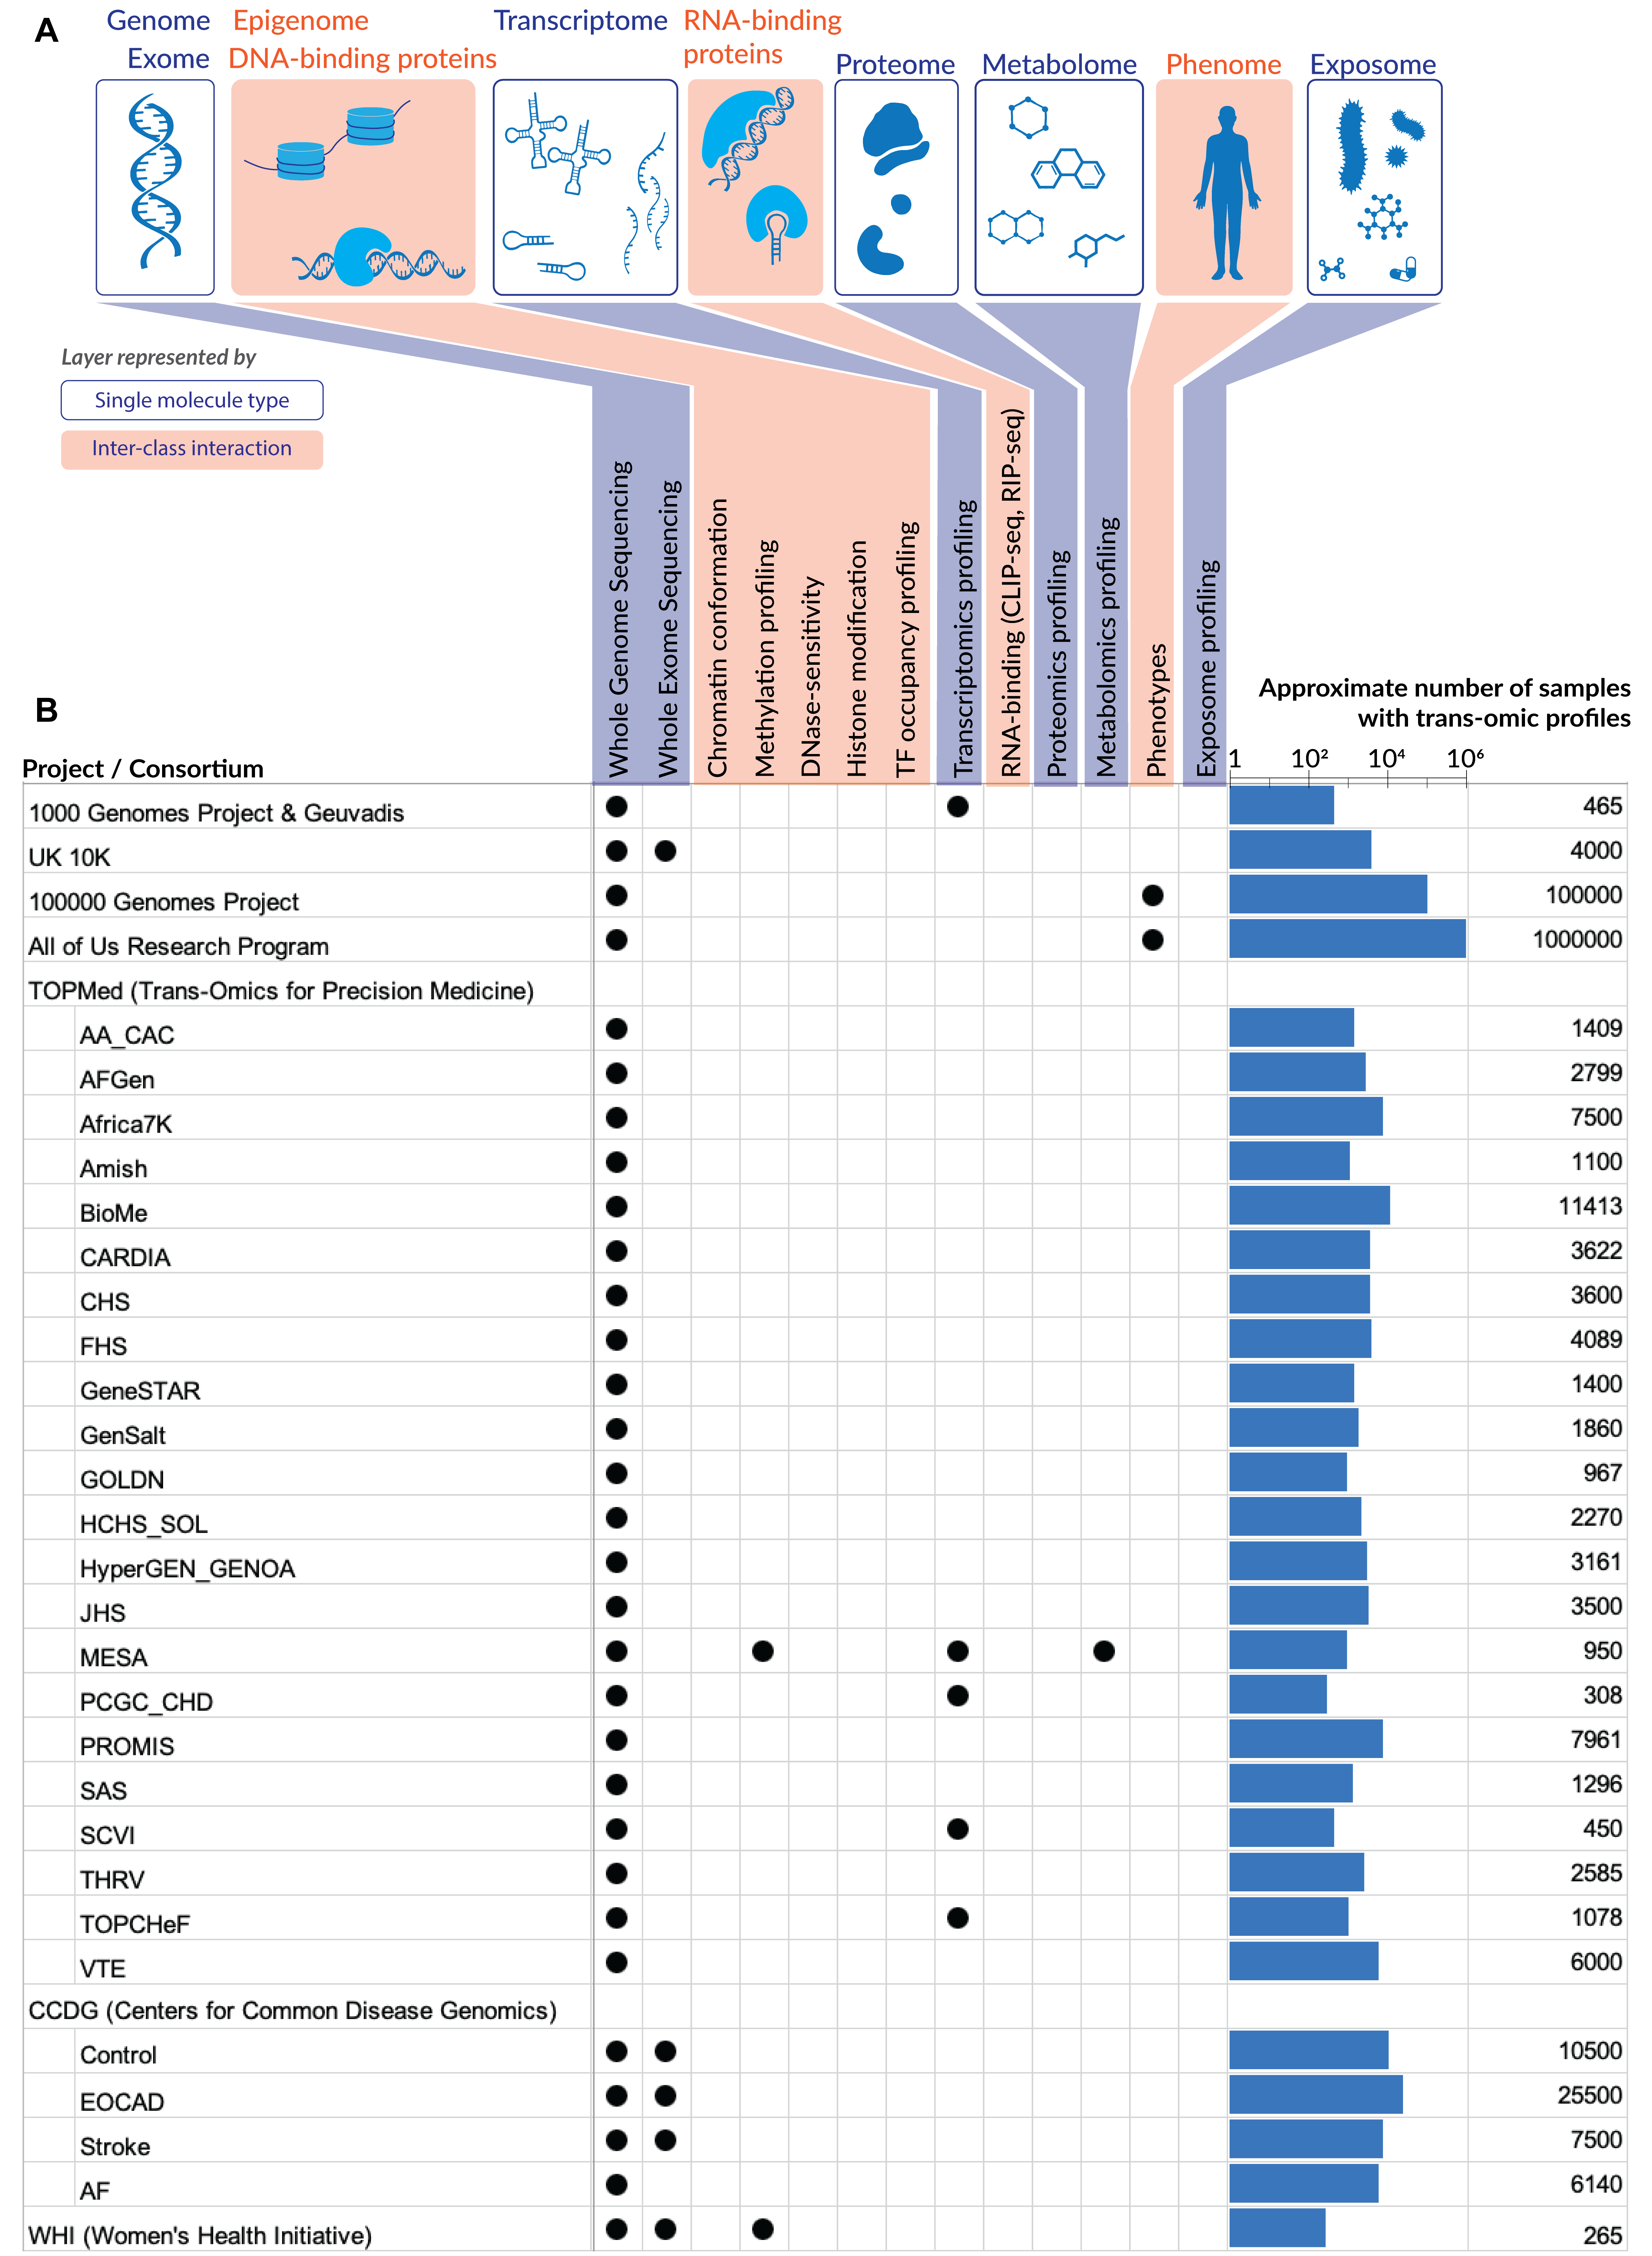
\includegraphics[width=1\linewidth]{trans-omics-data-sets.png}
		\caption{Large omics data sets that are or will be available for CVD research, spanning all major classes of biomolecules: DNA, RNA, proteins and their interactions. For each data set, the number of samples being assayed across multiple omics are indicated on the right. This number is often smaller than the total number of samples/participants in a given project, because not every sample is run on multiple assays.}
		\label{fig:trans-omics}
	\end{figure*} 
	

	\begin{table}[]
	\processtable{The subject count aggregated from studies deposited in dbGaP, consented for General Research Use (GRU)
		\label{tab:dbgapSubject}}
{\begin{tabular}{l l l}
			\toprule
			& \textbf{CVD} &  \textbf{All}                         \\ \midrule
			16s rRNA (NGS)                 &     0 &      92 \\
			CNV Genotypes                  &     0 &   48972 \\
			Chromatin (NGS)                &     0 &     139 \\
			Genomic Sequence Amplicon (NGS)&     0 &       8 \\
			Methylation (CpG)              &     0 &     657 \\
			Methylome sequencing           &     0 &     152 \\
			QTL Results                    &     0 &     281 \\
			RNA Seq (NGS)                  &   333 &    1498 \\
			SNP Genotypes (Array)          &  6658 &  113597 \\
			SNP Genotypes (NGS)            &  4277 &   11786 \\
			SNP Genotypes (PCR)            &     0 &      10 \\
			SNP Genotypes (imputed)        &     0 &   29693 \\
			SNP/CNV Genotypes (NGS)        &     0 &     936 \\
			SNP/CNV Genotypes (imputed)    &     0 &    9291 \\
			SNV (.MAF)                     &     0 &       2 \\
			SNV Aggregate (.MAF)           &     0 &     570 \\
			Targeted Genome (NGS)          &     0 &    9918 \\
			Whole Exome (NGS)              &  5518 &   12771 \\
			Whole Genome (NGS)             &     0 &    1245 \\
			mRNA Expression (Array)        &     0 &     798 \\
			miRNA (NGS)                        & 0 &   228 \\ \hline
			Total subject count in data consented for GRU & 16786 & 242644 \\ \hline
			All consent groups & 658305 & Unknown \\	
		\end{tabular}}{NGS: Next-generation sequencing\\ QTL: Quantitative Trait Loci}
	\end{table}
	
	
	\subsection*{Infrastructure considerations}
	Large amounts of data impose critical challenges in storing, managing and computing. The Sequence Read Archive (SRA) \citep{Leinonen:2011:Sequence} is now home to 14 petabytes of sequencing data from over 100,000 studies \citep{Langmead:2018:Cloud}.
	Although the storage required to store the raw output of high-throughput sequencing experiments are certainly exceeding the capability of an average computing facility, the major challenge is turning these archives into easily accessible databases, especially under the legal and ethical requirements to protect participants' privacy.
	As illustrated in Table \ref{tab:dbgapSubject}, there are 658,305 records of genotype-phenotype data potentially relevant to future biomedical studies. To access these data, one needs to file a request, prepare the facility, implement the security measures, and transfer the data upon approval. However, before filing a request, one needs to dive into the metadata of individual studies and decide which datasets are useful for the target research. Important information about a dataset such as the list of phenotypic variables are vastly different from study to study and cannot be filtered against. In addition to those parameters of a study design, researchers need to be aware of the various types of consents applied to different datasets, many times within a single study. This procedure to obtain data access is currently applied for all controlled-access data in dbGaP, adding a significant administrative burden to biomedical researchers.
	As an effort towards more accessible biomedical data, the AHA's Precision Medicine Platform \citep{Kass-Hout:2018:American} has simplified this process by streamlining the search, request and transfer of data. Datasets deposited on the platform were harmonized such that users can query for data across multiple studies by some common parameters, selectively request access to the relevant data, and perform analyses on the cloud-based workspace.
	Although the data filtering step is greatly facilitated, data can only be delivered to a restricted community who has been granted access and becomes responsible for securing their copy of the controlled-access data. In the attempt to alleviate all the responsibilities associated with the direct access of sensitive data, the DataSHIELD platform was developed \citep{Gaye:2014:DataSHIELD, Wilson:2017:DataSHIELD}. This platform allows data users to perform analytics without disclosure of sensitive or identifiable information.
	%more applications \citep{Wilson:2017:DataSHIELD}.  
	In parallel to these efforts, bioinformatics analyses have also started to benefit from cloud-based computing, where a number of projects have successfully re-processed and re-analyzed the large amount of biological samples across large databases such as TCGA, dbGaP, etc., providing novel insights or cloud-compatible analytic protocols, such as Rail-dbGaP \citep{Nellore:2016:RaildbGaP}, Toil \citep{Vivian:2017:Toil}, and ENCORE \citep{UMich:2018:Encore}. These successes on one hand demonstrate the great potential of existing datasets, and on the other, provide concrete examples on how cloud-based computing can be performed to overcome huge requirements of storage, memory and computational power. More than 20 providers are provisioning cloud services in both commercial and academic sectors \citep{Langmead:2018:Cloud}, promising even lower costs and higher accessibility.
	
	
	%Guidelines, protocol
	%Data visibility
	%efforts to standardize data management and sharing
	%
	
	\subsection*{Perspectives -- past and present}
	
	As early as 1999 when the complete human genome and high-throughput transcriptomic profiling were still on the horizon, research communities had started to recognize the critical use of bioinformatic analyses in generating insights from these kinds of data. For example, the computational approaches outlined by \cite{Claverie:1999:Computational} for the early day gene expression data are still popular in today's transcriptomics studies: differential gene expression analysis, co-expression analysis and gene clustering with subsequent identification of enriched biological pathways. Those old-fashioned methods can still bring fruitful analyses, as illustrated in a recent study on heart failure \citep{Santolini:2018:personalized}. These days, with more samples piling up from individual studies, such analyses can be performed with much higher statistical power.
	
	As high-throughput technology expanded to cover different molecular aspects of cellular processes, the potential power of integrative analysis on multiple layers of -omics data was recognized as early as a decade ago \citep{Hawkins:2010:Nextgeneration}. Since then, various strategies have been developed, following one of two schemes: multi-staged or meta-dimensional (\cite{Ritchie:2015:Methods}). Multi-staged data integration has been routinely used in cardiovascular research, for example in transcriptome-wide association studies (TWAS) where expression quantitative trait (eQTL) loci and GWAS-based SNPs are tested for correlation with gene expression levels from transcriptomic profiling data. Meta-dimensional data integration does not rely on the assumption that phenotype is the end point of the one-way flow of information from genome, to transcriptome and then proteome, thus allowing for modeling of complex phenotype without prior knowledge about the interplay of different omics layers.
	\comment{find examples -- in and outside of CVDs}
	
	%* proteomics + transcriptomics \citep{Uhlen:2015:Tissuebased}
	%
	%* genomics + transcriptomics \citep{Klarin:2017:Genetic}

	
	

	%In clinical application, the focus is on facilitating clinical decisions.
	
	%Visualization of chromatin 3D structure emerges as a demand to analyze and present experimental data from conformation capture experiments. The challenges posed by these experiments, being new, high-throughput and  3-dimensional, are actively researched visualization problems \citep{Goodstadt:2017:Challenges}. As a researcher in cardiovascular disease, it is important to stay abreast with the developments in this field to make the most use of the available data.
	
	
	
	%Most often, the bottleneck in the application of these computational methods are not in their implementation, but in the shortage of domain knowledge. Many generic bio-portals have been published in the recent years, aiming to make complicated data as accessible as possible to a general audience. The lack of focus on a research topic has limited their usefulness.
	
	%%%%%% perspective


	
	%\subsection{Prospective development}
	
	%nanopore sequencing
	
	%single cell
	
	\section*{Notes section}
	
	Although not a traditional part of computational research, visualization has become indispensable in data-driven research, facilitating biological research in data exploration, pattern recognition, and data representation. Visualization methods are blooming to accommodate the diverse data types in biology \citep{Pavlopoulos:2015:Visualizing}. In this arena, the exciting challenge to cardioinformatics researchers is how to integrate and represent data layers in a meaningful manner.
		
		
	Search engine and knowledge synthesis \citep{Lutjohann:2011:Sciencenet}. A universal element of all research, knowledge synthesis is under-rated research task. Like most other areas, most of the work in knowledge synthesis has been and has to be done manually in cardiovascular research. Cardiovascular diseases impose the challenge of understanding complex systems of multiple dimensions, creating the pressing need of summarizing and synthesizing knowledge from the vast body of research in a more robust manner. \comment{Natural language processing?}
		
		
	
	Maybe mention ExAC and gnomAD browsers for ancestry, which include rs IDs involved in CVD, although it's not a pressing issue to mention.
	
	The first draft of the human genome project had brought a lot of hope and excitement about potential advancements in the diagnosis and treatment of cardiac diseases, such as the ability to identify disease genes within the associated loci, to improve risk estimation based on more precise genotypes, or to personalize the prediction of drug effect on a patient, \citep{Komajda:2001:heart}.
	
	
	Outstanding problems
	
	Variant calling and pathogenicity prediction. Currently inconsistent. Mostly developed for protein-coding fraction of the genome (SIFT, Polyphen, etc.), largely ignore the non-coding regions.
	Pathogenicity assignment: variable, conflicting, not applicable for all populations.
	
	Risk estimation
	
	Lack of mechanistic understanding
	
	Lack of platforms for accessible data and knowledge base
	
	%{https://www.ncbi.nlm.nih.gov/mesh/68002318} 
	
	As we further our quest to understand the genetics of heart diseases, many conditions have become too complicated for traditional approaches. Reflecting on the current body of knowledge, we recognize that many aspects of this complexity can be addressed with more computational methods.
	
	
	\comment{Trang -- cite these somewhere:} CardioGenBase, OmicsDI.
	
	
	
\section*{Closing remarks}
Bioinformatics is more than just a powerful toolkit of techniques for conducting high-end cardiovascular disease research, as important perspectives have arisen from the application, development, and expansion of advanced computational methodologies.  In this review, we discussed some of the important work happening at the multidisciplinary interface of bioinformatics and cardiology, and advocated for shining a brighter spotlight on cardioinformatics as an emerging field, in its own right.  We suggested some future insights based on our understanding of historical perspectives and ongoing work in current CVD research, and we welcome feedback and ideas from the broader scientific community.
	
	%
	
	\enlargethispage{12pt}
	
	
	
	
	\section*{Acknowledgements}
	
	BBK acknowledges and thanks the American Heart Association (AHA) for financial support through the AHA Postdoctoral Fellowship program.
	\vspace*{-12pt}
	
	\section*{Funding}
	
	This work has been supported by the American Heart Association (AHA) Postdoctoral Fellowship grant \#18POST34030375 (Khomtchouk).\vspace*{-12pt}
	
	\bibliographystyle{natbib}
	%\bibliographystyle{achemnat}
	%\bibliographystyle{plainnat}
	%\bibliographystyle{abbrv}
	%
	%\bibliographystyle{plain}
	%
	\bibliography{cardio}
	
	
	
\end{document}